\documentclass[../ZF_SWEN1.tex]{subfiles}
\begin{document}

\begin{figure}[H]
\centering
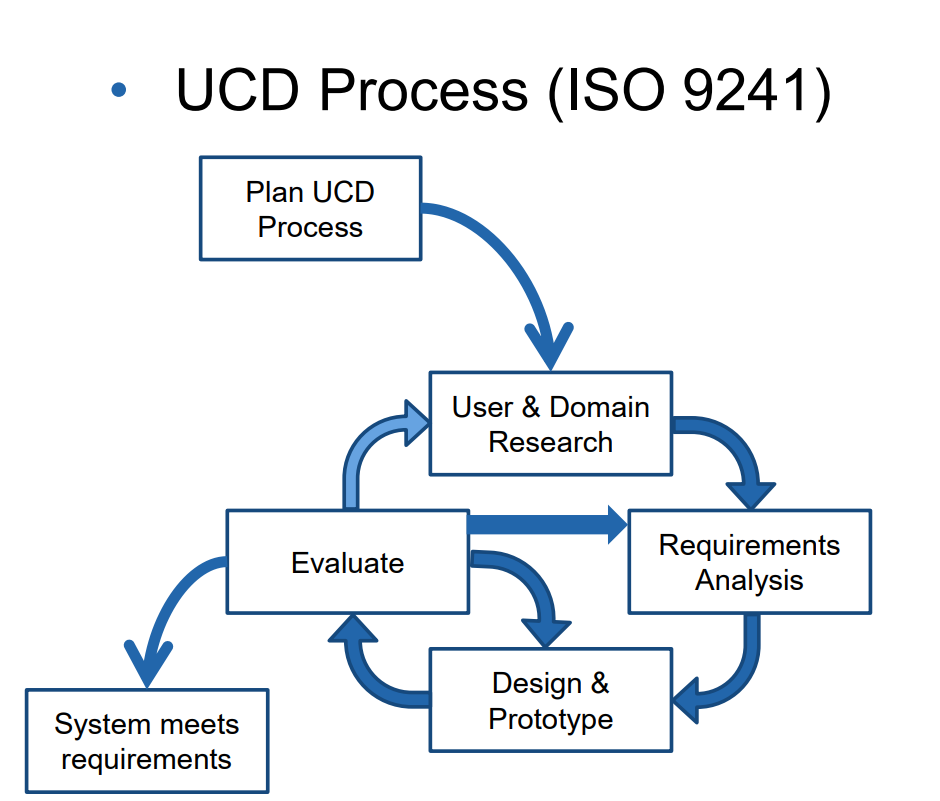
\includegraphics[width=0.3\textwidth]{Resources/Images/UCD_Process.png}
\caption{\label{fig:UCDProcess} UCDProcess}
\end{figure}

\subsection{User \& Domain Research}
\begin{itemize}
	\item \textcolor{red} {\textbf{Ziele bez. Benutzer:}}
	\begin{itemize}
		\item Wer ist Benutzer
		\item Was ist die Arbeit (Aufgaben, Ziele)
		\item Wie sieht Arbeitsumgebung aus
		\item Was wird gebraucht um Ziele zu erreichen
	\end{itemize}
	\item Welche Sprache, Begriffe
	\item Normen (organisatorisch, kulturell, sozial)
	\item Pain Points (Brüche, Workarounds)
	\item Für mobile Apps:
	\begin{itemize}
		\item Nutzungskontext
		\begin{itemize}
			\item Wo wird App benutzt (Umgebung)
			\item Wann wird App benutzt (Tageszeit, involvierte Personen, Randbedingungen)
			\item Warum wird App benutzt (Nutzen, Motivation, Trigger)
		\end{itemize}
	\end{itemize}
	\item \textcolor{red} {\textbf{Ziele bez. Domäne:}}
	\begin{itemize}
		\item Buisiness der Firma verstehen
		\item Domäne verstehen (Sprache, Wichtigste Konzepte, Prozesse)
	\end{itemize}
	
\end{itemize}

\subsubsection{GUI Design Process}
\paragraph{Methoden User \& Domain Research}
\begin{itemize}
	\item Contextual Inquiry
	\begin{itemize}
		\item Was ist das?(Beobachtung, Interview)
		\item Was braucht es dazu? (Für den inquiry, z.B Videogerät)
	\end{itemize}
	\item Interviews
	\item Beobachtung
	\item Fokusgruppen
	\item Umfragen
	\item Nutzungsauswertung
	\item Desktop Research (Dokumentenstudium, Mitbewerber)
\end{itemize}


\subsubsection{Wichtige Artekfakte}
\begin{itemize}
	\item \textcolor{pink}{\textbf{Personas}}
	\item \textcolor{pink}{\textbf{Usage-Szenarien}}
	\begin{itemize}
		\item Kurze Geschichte
		\begin{itemize}
			\item \textcolor{green} {Usage Szenarien}
			\begin{itemize}
				\item aktuelle Situation
				\item in User and domain research verwendet
			\end{itemize}
			\item \textcolor{green} {Kontextszenarien}
			\begin{itemize}
				\item Zukünftige gewünschte Situation
				\item in Anforderungsanalyse verwendet
			\end{itemize}
		\end{itemize}
		
	\end{itemize}
	\item \textcolor{pink}{\textbf{Mentales Modell}}
	\item \textcolor{pink}{\textbf{Domänenmodell}}
	\item \textcolor{pink}{\textbf{Stakeholder Map}}
	\begin{figure}[H]
	\centering
	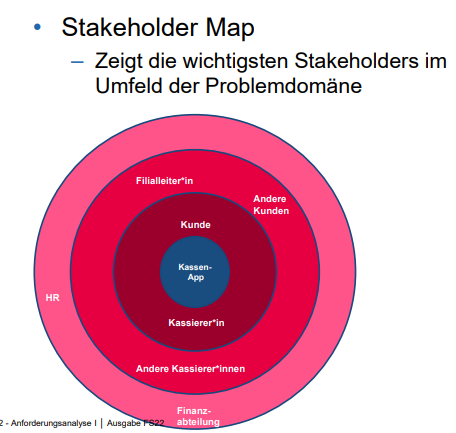
\includegraphics[width=0.3\textwidth]{Resources/Images/Stakeholdermap.png}
	\caption{\label{fig:Stakeholdermap} Stakeholdermap}
	\end{figure}
	\item \textcolor{pink}{\textbf{Service Blueprint/Geschäftsprozessmodell}}
	\begin{figure}[H]
	\centering
	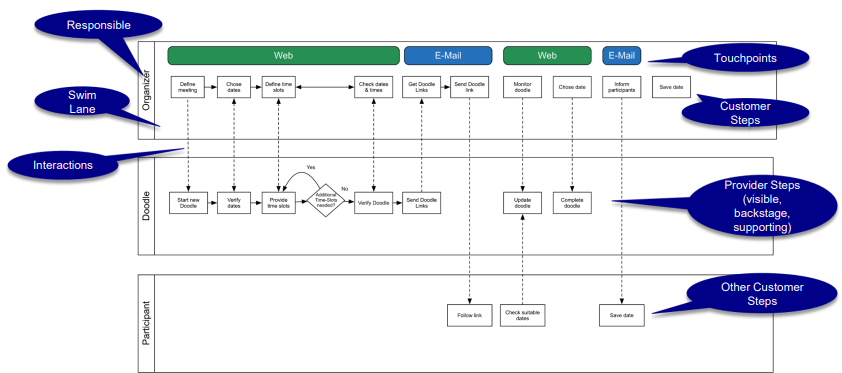
\includegraphics[width=0.3\textwidth] {Resources/Images/Blueprint.png}
	\caption{\label{fig:Blueprint}Blueprint}
	\end{figure}
	
\end{itemize}
\subsection{Anforderungsanalyse}

\textbf{Ziel:}\\
\begin{itemize}
	\item Ausgehend von den Resultaten des UCD -$>$ User-Anforderungen ableiten:
	\begin{itemize}
		\item Funktionale Abläufe, Interaktionen 
		\begin{itemize}
			\item \textcolor {gray} {\textbf{Kontextszenarien}}
			\item \textcolor {gray} {\textbf{Storyboards}}
			\item \textcolor {gray} {\textbf{UI-Skizzen}}
			\item \textcolor {gray} {\textbf{Use cases}}
		\end{itemize}
		\item Konzepte, Beziehungen, Quantitäten
		\begin{itemize}
			\item \textcolor {gray} {\textbf{Kontextszenarien}}
		\end{itemize}
		\begin{itemize}
			\item \textcolor {gray} {\textbf{FURPS-Modell (Functionality, Usability, Reliability, Performance, Supportablility}}
		
		\end{itemize}				
		
	\end{itemize}
\end{itemize}

\subsubsection{Use Cases}

\begin{itemize}
	\item \colorbox {green!30}{\textbf{Akteur}}
	\begin{itemize}
		\item Primärakteur
		\item Unterstützender Akteur
		\item Offstage-Akteur
	\end{itemize}
	\item \colorbox {green!30}{\textbf{Keine Kann-Formulierungen}}
	\item \colorbox {green!30}{\textbf{3 Ausprägungen:}}
	\begin{enumerate}
		\item Kurz
		\begin{itemize}
			\item Titel + 1 Absatz (Standardablauf)
		\end{itemize}
		\item Informell
		\begin{itemize}
			\item Titel + Informelle Beschreibung (können mehrere Absätze sein, beschreibt auch Varianten)
		\end{itemize}
		\item Vollständig
		\begin{itemize}
			\item Titel + alle Schritte und alle Varianten im Detail
			\item UC-Name
			\item Umfang
			\item Ebene
			\item Primärakteur
			\item Stakeholders und Interessen
			\item Vorbedingungen
			\item Erfolgsgarantie/Nachbedingungen
			\item Standardablauf
			\item Erweiterungen
			\item Spezielle Anforderungen
			\item Liste der Technik und Datavariationen
			\item Häfigkeit des Auftretens
			\item Verschiedenes
		\end{itemize}
		
	\end{enumerate}
	\item \colorbox {green!30}{\textbf{Notation = Nomen + Verb}}
\end{itemize}

\subsubsection{Wie schreibt man Use Cases}

\colorbox {orange!30}{\textbf{Brief UC:}}
\begin{itemize}
	\item Kurze Beschreibung des Anwendungsfalls in einem Paragraph
	\begin{itemize}
		\item Nur Erfolgszenario
		\item Sollte enthalten:
		\begin{itemize}
			\item Trigger des UCs
			\item Akteure
			\item summarischen Ablauf des UCs
		\end{itemize}
		\item Zu beginn der Analyse
	\end{itemize}
\end{itemize}

\colorbox {orange!30}{\textbf{Casual UC:}}
\begin{itemize}
	\item Informelle Beschreibung des Anwendungsfalls in mehreren Paragraphen
	\begin{itemize}
		\item Nur Erfolgszenario + wichtigste Alternativszenarien
		\item Sollte enthalten:
		\begin{itemize}
			\item Trigger des UCs
			\item Akteure
			\item Interaktion Akteurs mit System
		\end{itemize}
		\item Zu beginn der Analyse
	\end{itemize}
\end{itemize}
\colorbox {orange!30}{\textbf{Fully-dressed UC:}}
\begin{itemize}
	\item Detaillierte Beschreibung des ablaufs mit allen Alternativszenarien

		\item ende der Inception und v.a. in Elaborationphase
		\item Die wichtigsten UCs(10\%), die die Architektur bestimmen
\end{itemize}
\paragraph{\begin{Large}
	Formaler Aufbau:\\
\end{Large}}
\begin{enumerate}
	\item 
		\begin{large}
			\colorbox{teal!30}{\textbf{UC-Name}}
		\end{large}
	\begin{itemize}
		\item Aktiv formulieren (Verb + ev.Objekt)
		\item Beschreibt Job(Ziel,Aufgabe),den Akteur ausführen will
	\end{itemize}
	\item	
		\begin{large}
			\colorbox{teal!30}{\textbf{Umfang(Scope)}}
		\end{large}
	\begin{itemize}
		\item Beschreibt das zu entwickelnde System (SuD= System under Development)
	\end{itemize}
	\item 
	\begin{large}
		\colorbox{teal!30}{\textbf{Ebene(Level)}}
	\end{large}
	\begin{itemize}
		\item Anwenderziel oder
		\item Subfunktion
	\end{itemize}
	\item 
	\begin{large}
		\colorbox{teal!30}{\textbf{Primärakteur}}
	\end{large}
	\begin{itemize}
		\item Hauptakteur des UCs
		\begin{itemize}
			\item Primärer Nutzniesser des UC
			\item initiiert den UC
			\item Interagiert hauptsächlich mit dem System
		\end{itemize}
	\end{itemize}
	\item
	\begin{large}
		\colorbox{teal!30}{\textbf{Stakeholders und Interessen}}
	\end{large}
	\begin{itemize}
		\item Für wen ist der UC sonst noch relevant und welche Interessen hat er daran?
	\end{itemize}
	\item \begin{large}
		\colorbox{teal!30}{\textbf{Vorbedingungen(Preconditions)}}
	\end{large}
	\begin{itemize}
		\item Was ist die unmittelbare Voraussetzung, damit UC ablaufen kann? (Nur die wichtigsten,offensichtliche Voraussetzungen)
	\end{itemize}
	\item 	
	\begin{large}
		\colorbox{teal!30}{\textbf{Erfolgsgarantie/Nachbedingungen(Success Guarantee)}}
	\end{large}
	\begin{itemize}
		\item Was muss gewährleistet sein nach erfolgreichem Ablauf von UC
	\end{itemize}
	\item 
	\begin{large}
		\colorbox{teal!30}{\textbf{Standardablauf (Main Success Scenario)}}
	\end{large}
	\begin{itemize}
		\item Wichtigster Teil des UCs(Beschreibung erfolgreichen Ablaufs des UCs)
		\item Beschreibung Interaktion Primärakteurs mit dem System(+allenfalls Interaktion mit unterstützenden Akteuren)
		\item Startpunkt= nach den Vorbedingungen
		\item Keine Lösungsdetails
	\end{itemize}
	\item 
	\begin{large}
		\colorbox{teal!30}{\textbf{Erweiterungen (Extensions)}}
	\end{large}
	\begin{itemize}
		\item Alternative Erfolgs-aber auch Misserfolgszenarien
		\item Erweiterungen / alternative Abläufe
		\item * = Alternativablauf zu jeder Zeit auftreten kann
		\item Interaktion des alternativen Ablaufs analog zu Hautptszenario
		\item 			\begin{figure}[H]
			\centering
			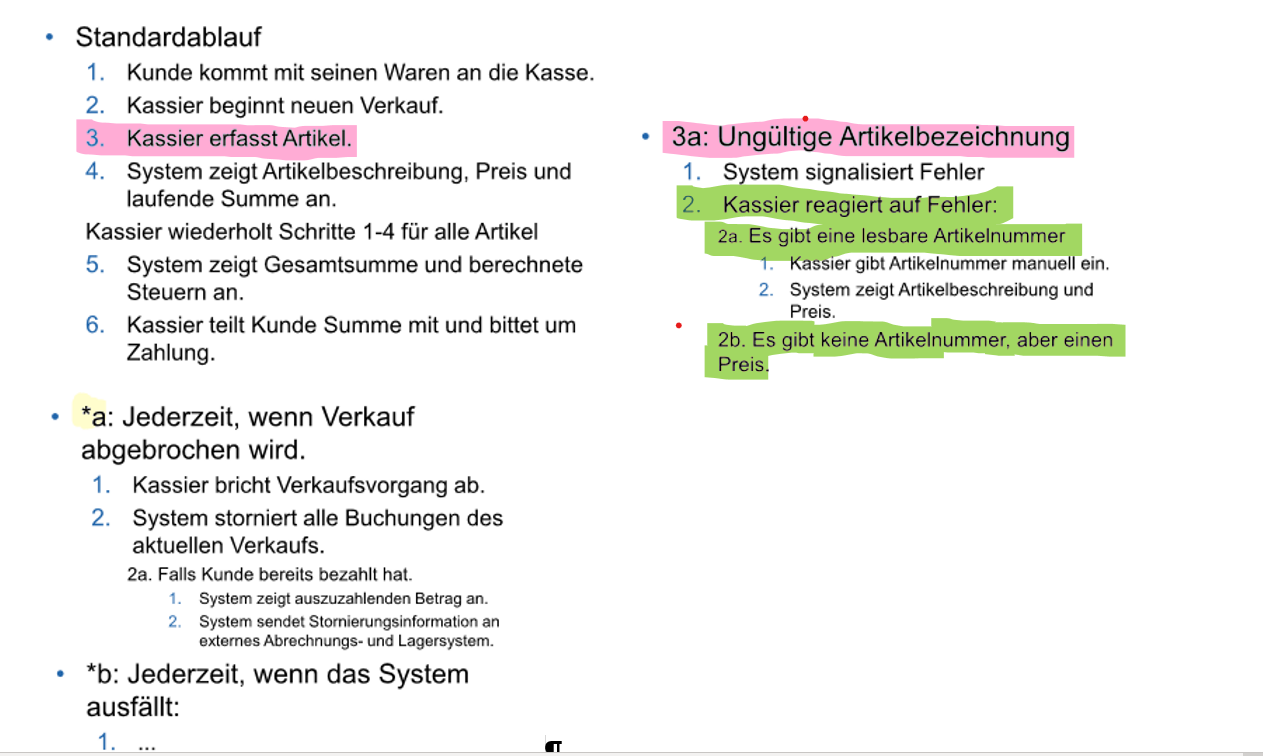
\includegraphics[width=0.3\textwidth]{Resources/Images/Beispiel-Fully-Dressed.png}
			\caption{\label{fig:Beispiel-Fully-Dressed}Beispiel-Fully-Dressed.}
		\end{figure}
	\item 
	\begin{large}
		\colorbox{teal!30}{\textbf{Spezielle Anforderungen (Special Requirements)}}
	\end{large}
	\begin{itemize}
		\item Weitere Anforderungen, die aus diesem UC resultieren
	\end{itemize}
	\item 
		\begin{large}
			\colorbox{teal!30}{\textbf{Liste der Technik und Datavariationen (Technology and Data Variations)}}
		\end{large}
	\begin{itemize}
		\item Alternative I/O-Methoden, Datenformate, etc.(Notation wie bei Erweiterung)
	\end{itemize}
	\item 
	\begin{large}
		\colorbox{teal!30}{\textbf{Häufigkeit des Auftretens(Frequency of Occurance)}}
	\end{large}
	\begin{itemize}
		\item Wie häufig tritt dieser UC auf?
	\end{itemize}
	\item 
	\begin{large}
		\colorbox{teal!30}{\textbf{Verschiedenes (Miscellaneous)}}
	\end{large}
	\begin{itemize}
		\item Offene Fragen/ Probleme
	\end{itemize}
\end{itemize}
		
\end{enumerate}
\paragraph{von Anwendungsfällen zu konkreten Funktionalitäten:}
\begin{itemize}
	\item Systemsequenzdiagramme
	\item Operation Contracts
\end{itemize}
\subsubsection{UML Sequenzdiagramm (SSD)}

\paragraph{Zeigt:} Interaktion der Akteure mit dem System
\begin{itemize}
	\item Welche Input-Events auf das System einwirken
	\item Welche Output-Events das System erzeugt
\end{itemize}
SSD können auch Interaktionen zwischen SuD und externen unterstützenden System zeigen.

\paragraph{Ziel:} Wichtigste Systemoperationen identifizieren, die das System zur Verfügung stellen muss (API) für einen gegebenen Anwendungsfall



\paragraph{Wie Systemoperationen finden:}
\begin{enumerate}
	\item Szenario für UC Schritt für Schritt durchgehen
	\item Für jeden Schritt Systemoperation überlegen
	\begin{itemize}
		\item Geeigneten, präzisen Namen wählen (POV Akteur)
		\item Welche Info braucht das System um Systemop. auszuführen? (Wenn nicht vorhanden im System -$>$ Parameter)
	\end{itemize}
\end{enumerate}

\subsubsection{Operation Contract}

\textbf{Definition: } Spezifiziert (System)Operation \\

\begin{itemize}
	\item Name plus Parameterliste
	\item Vorbedingung (Was muss zwingend erfüllt sein damit Systemoperation aufgerufen werden kann)
	\item Nachbedingung
	\begin{itemize}
		\item Was hat sich alles geändert nach Ausführung (Erstellte / gelöschte Instanzen, Assoziationen, geänderte Attribute), Im Präsens schreiben
		\item basierend auf Domänenmodell
	\end{itemize}
\end{itemize}


\paragraph{Wann Operation Contracts?}
\begin{itemize}
	\item Nur wenn aus Anwendungsfall nicht klar wird, was Systemoperation genau machen muss
	\begin{itemize}
		\item Meist nur bei sehr komplizierten Operationen und/oder
		\item Wenn Entwicklung der Systemoperation ausgelagert wird
	\end{itemize}
	\item Erst gegen Ende des Meilensteins Lösungsarchitektur oder kurz vor Start des Designs der Systemoperation
\end{itemize}


\subsubsection{Zusätzliche Anforderungen}

\begin{itemize}
	\item weitere Funktionale (grosser Teil schon von UCs beschrieben)
	\item Nicht-Funktionale
\end{itemize}


\paragraph{Formulierung}

\begin{itemize}
	\item Anforderungstatements
	\begin{itemize}
		\item Als Anforderung formuliert
		\item messbar/verifizierbar
	\end{itemize}
	\item So wenig wie nötig
	\begin{itemize}
		\item Nur diejenige, die begründet gefordert werden
		\item Keine ersten Lösungsideen als Forderungen
	\end{itemize}
	\item User-Stories
	\begin{itemize}
		\item In einem Satz wer,was,warum fordert
		\item Erfüllen einige Bedingungen automatisch
		\item die anderen Bedingungen (Messbarkeit etc.) solten auch erfüllt sein
	\end{itemize}
\end{itemize}


\paragraph{Checkliste FURPS+}

\begin{itemize}
	\item \textbf Functionality
	\begin{itemize}
		\item Features, Fähigkeiten, Sicherheit
	\end{itemize}
	\item \textbf Usability
	\begin{itemize}
		\item Usability Anforderungen (Kap.5.3)
		\item Accessibility
	\end{itemize}
	\item \textbf Reliability
	\begin{itemize}
		\item Fehlerrate, Wiederanlauffähigkeit, Vorhersagbarkeit, Datensicherung
	\end{itemize}
	\item \textbf Performance
	\begin{itemize}
		\item Reaktionszeiten, Durchsatz, Genauigkeit, Verfügbarkeit, Ressourceneinsatz
	\end{itemize}
	\item \textbf Supportability
	\begin{itemize}
		\item Anpassungsfähigkeit, Wartbarkeit, Internationalisierung, Konfigurierbarkeit
	\end{itemize}
	\item \textbf {+}
	\begin{itemize}
		\item Implementation (HW,BS,Sprachen, Tests...)
		\item Interface
		\item Operations
		\item Packaging
		\item Legal
	\end{itemize}
\end{itemize}


\paragraph{Glossar}

\begin{itemize}
	\item Einfaches Glossar
	\begin{itemize}
		\item Begriffe im Projekt und SW-Produkt
		\item beliebige Elemente 
	\end{itemize}
	\item Data Dictionary
	\begin{itemize}
		\item Zusätzliche Datenformate, Wertebereiche, Validierungsregeln
	\end{itemize}
\end{itemize}






















































\end{document}